\documentclass{standalone}
\usepackage{tikz}
\usetikzlibrary{patterns, positioning}

\begin{document}
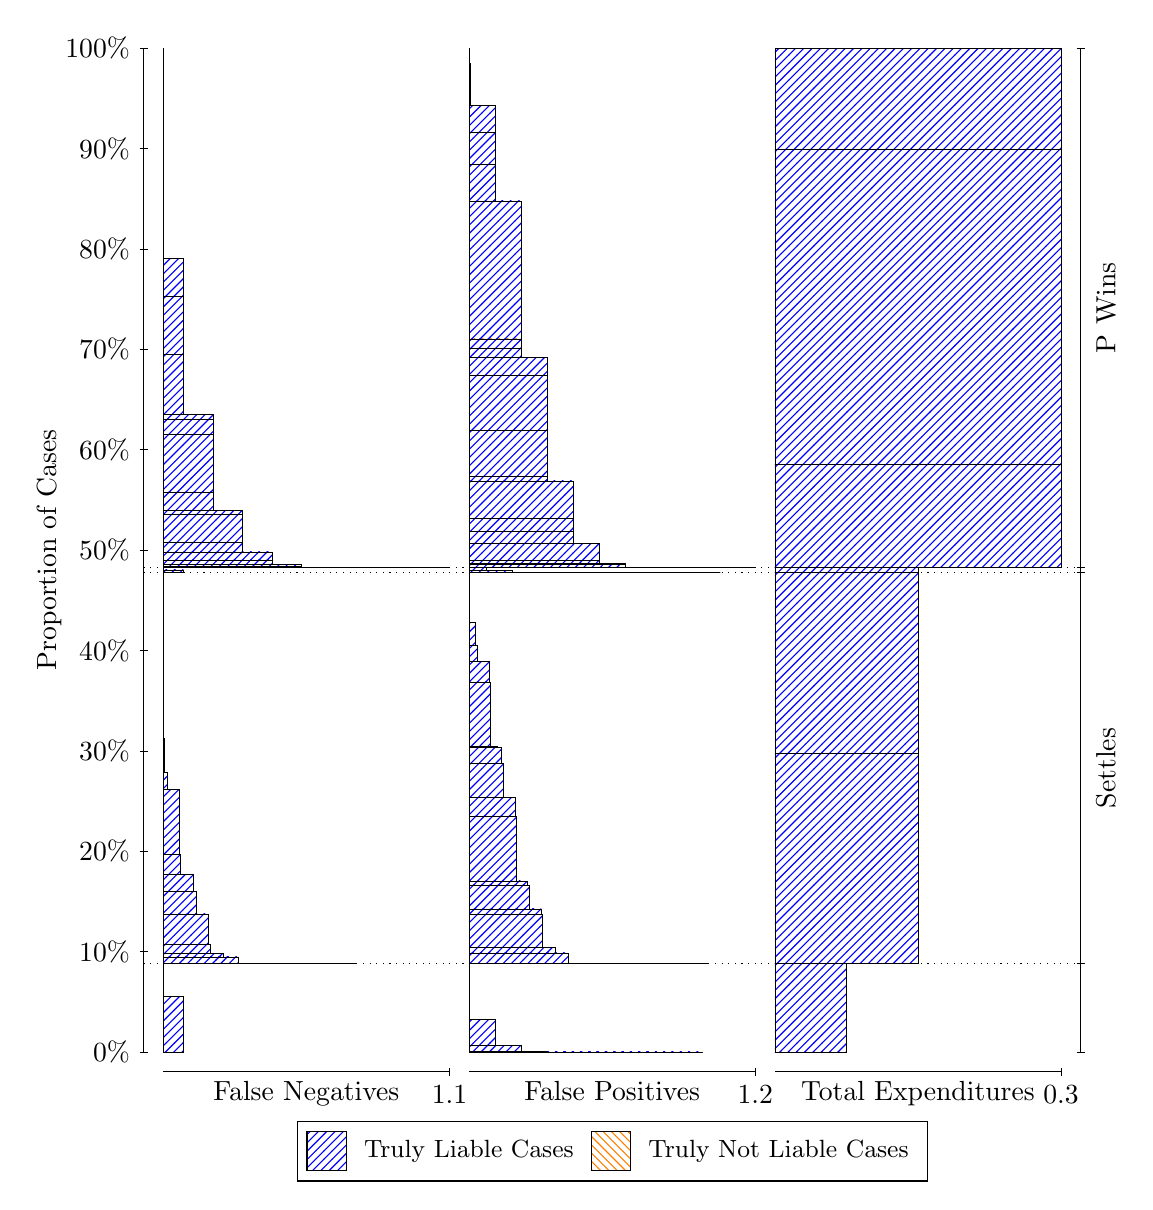
\begin{tikzpicture}
\draw[black, very thin] (1.5,1.75) -- (1.5,14.5);
\node[rotate=90, anchor=center] at (0.3, 8.125) {Proportion of Cases};
\draw[black, very thin] (1.45,1.75) -- (1.55,1.75);
\node[anchor=east] at (1.45, 1.75) {0\%};
\draw[black, very thin] (1.45,3.025) -- (1.55,3.025);
\node[anchor=east] at (1.45, 3.025) {10\%};
\draw[black, very thin] (1.45,4.3) -- (1.55,4.3);
\node[anchor=east] at (1.45, 4.3) {20\%};
\draw[black, very thin] (1.45,5.575) -- (1.55,5.575);
\node[anchor=east] at (1.45, 5.575) {30\%};
\draw[black, very thin] (1.45,6.85) -- (1.55,6.85);
\node[anchor=east] at (1.45, 6.85) {40\%};
\draw[black, very thin] (1.45,8.125) -- (1.55,8.125);
\node[anchor=east] at (1.45, 8.125) {50\%};
\draw[black, very thin] (1.45,9.4) -- (1.55,9.4);
\node[anchor=east] at (1.45, 9.4) {60\%};
\draw[black, very thin] (1.45,10.675) -- (1.55,10.675);
\node[anchor=east] at (1.45, 10.675) {70\%};
\draw[black, very thin] (1.45,11.95) -- (1.55,11.95);
\node[anchor=east] at (1.45, 11.95) {80\%};
\draw[black, very thin] (1.45,13.225) -- (1.55,13.225);
\node[anchor=east] at (1.45, 13.225) {90\%};
\draw[black, very thin] (1.45,14.5) -- (1.55,14.5);
\node[anchor=east] at (1.45, 14.5) {100\%};

\draw[black, very thin] (13.4,1.75) -- (13.4,14.5);
\draw[black, very thin] (13.35,1.75) -- (13.45,1.75);
\node[anchor=west] at (13.35, 1.75) {};
\draw[black, very thin] (13.35,2.8721) -- (13.45,2.8721);
\node[anchor=west] at (13.35, 2.8721) {};
\draw[black, very thin] (13.35,7.838) -- (13.45,7.838);
\node[anchor=west] at (13.35, 7.838) {};
\draw[black, very thin] (13.35,7.9018) -- (13.45,7.9018);
\node[anchor=west] at (13.35, 7.9018) {};
\draw[black, very thin] (13.35,14.5) -- (13.45,14.5);
\node[anchor=west] at (13.35, 14.5) {};

\draw[black, very thin, pattern color=blue, pattern=north east lines] (1.75,1.75) rectangle (2.0035,2.4561);
\draw[black, very thin, pattern color=orange, pattern=north west lines] (1.75,2.4561) rectangle (1.75,2.4561);
\draw[black, very thin, pattern color=blue, pattern=north east lines] (1.75,2.4561) rectangle (1.75,2.8721);
\draw[black, very thin, pattern color=blue, pattern=north east lines] (1.75,2.8721) rectangle (4.2004,2.8721);
\draw[black, very thin, pattern color=blue, pattern=north east lines] (1.75,2.8721) rectangle (3.8248,2.8721);
\draw[black, very thin, pattern color=blue, pattern=north east lines] (1.75,2.8721) rectangle (3.4493,2.8722);
\draw[black, very thin, pattern color=blue, pattern=north east lines] (1.75,2.8722) rectangle (3.3554,2.8722);
\draw[black, very thin, pattern color=blue, pattern=north east lines] (1.75,2.8722) rectangle (3.1864,2.8722);
\draw[black, very thin, pattern color=blue, pattern=north east lines] (1.75,2.8722) rectangle (3.0738,2.8776);
\draw[black, very thin, pattern color=blue, pattern=north east lines] (1.75,2.8776) rectangle (2.9799,2.8776);
\draw[black, very thin, pattern color=blue, pattern=north east lines] (1.75,2.8776) rectangle (2.8109,2.8776);
\draw[black, very thin, pattern color=blue, pattern=north east lines] (1.75,2.8776) rectangle (2.6982,2.9571);
\draw[black, very thin, pattern color=blue, pattern=north east lines] (1.75,2.9571) rectangle (2.6043,2.9572);
\draw[black, very thin, pattern color=blue, pattern=north east lines] (1.75,2.9572) rectangle (2.5105,3.0018);
\draw[black, very thin, pattern color=blue, pattern=north east lines] (1.75,3.0018) rectangle (2.4354,3.0018);
\draw[black, very thin, pattern color=blue, pattern=north east lines] (1.75,3.0018) rectangle (2.3415,3.1143);
\draw[black, very thin, pattern color=blue, pattern=north east lines] (1.75,3.1143) rectangle (2.3227,3.5028);
\draw[black, very thin, pattern color=blue, pattern=north east lines] (1.75,3.5028) rectangle (2.2288,3.5048);
\draw[black, very thin, pattern color=blue, pattern=north east lines] (1.75,3.5048) rectangle (2.1725,3.7917);
\draw[black, very thin, pattern color=blue, pattern=north east lines] (1.75,3.7917) rectangle (2.1349,4.0024);
\draw[black, very thin, pattern color=blue, pattern=north east lines] (1.75,4.0024) rectangle (2.0598,4.0028);
\draw[black, very thin, pattern color=blue, pattern=north east lines] (1.75,4.0028) rectangle (1.9659,4.2596);
\draw[black, very thin, pattern color=blue, pattern=north east lines] (1.75,4.2596) rectangle (1.9472,5.0822);
\draw[black, very thin, pattern color=blue, pattern=north east lines] (1.75,5.0822) rectangle (1.8533,5.0874);
\draw[black, very thin, pattern color=blue, pattern=north east lines] (1.75,5.0874) rectangle (1.7969,5.2994);
\draw[black, very thin, pattern color=blue, pattern=north east lines] (1.75,5.2994) rectangle (1.7594,5.731);
\draw[black, very thin, pattern color=orange, pattern=north west lines] (1.75,5.731) rectangle (1.75,5.731);
\draw[black, very thin, pattern color=blue, pattern=north east lines] (1.75,5.731) rectangle (1.75,7.838);
\draw[black, very thin, pattern color=blue, pattern=north east lines] (1.75,7.838) rectangle (2.0035,7.8713);
\draw[black, very thin, pattern color=orange, pattern=north west lines] (1.75,7.8713) rectangle (1.75,7.8713);
\draw[black, very thin, pattern color=blue, pattern=north east lines] (1.75,7.8713) rectangle (1.75,7.9018);
\draw[black, very thin, pattern color=blue, pattern=north east lines] (1.75,7.9018) rectangle (5.3833,7.9018);
\draw[black, very thin, pattern color=blue, pattern=north east lines] (1.75,7.9018) rectangle (5.0078,7.9018);
\draw[black, very thin, pattern color=blue, pattern=north east lines] (1.75,7.9018) rectangle (5.0078,7.9018);
\draw[black, very thin, pattern color=blue, pattern=north east lines] (1.75,7.9018) rectangle (4.6323,7.9018);
\draw[black, very thin, pattern color=blue, pattern=north east lines] (1.75,7.9018) rectangle (4.6323,7.9019);
\draw[black, very thin, pattern color=blue, pattern=north east lines] (1.75,7.9019) rectangle (4.2567,7.902);
\draw[black, very thin, pattern color=blue, pattern=north east lines] (1.75,7.902) rectangle (4.2567,7.9021);
\draw[black, very thin, pattern color=blue, pattern=north east lines] (1.75,7.9021) rectangle (3.8812,7.9057);
\draw[black, very thin, pattern color=blue, pattern=north east lines] (1.75,7.9057) rectangle (3.5056,7.9194);
\draw[black, very thin, pattern color=blue, pattern=north east lines] (1.75,7.9194) rectangle (3.5056,7.9381);
\draw[black, very thin, pattern color=blue, pattern=north east lines] (1.75,7.9381) rectangle (3.1301,7.9995);
\draw[black, very thin, pattern color=blue, pattern=north east lines] (1.75,7.9995) rectangle (3.1301,8.0898);
\draw[black, very thin, pattern color=blue, pattern=north east lines] (1.75,8.0898) rectangle (3.1301,8.1007);
\draw[black, very thin, pattern color=blue, pattern=north east lines] (1.75,8.1007) rectangle (2.7546,8.224);
\draw[black, very thin, pattern color=blue, pattern=north east lines] (1.75,8.224) rectangle (2.7546,8.5797);
\draw[black, very thin, pattern color=blue, pattern=north east lines] (1.75,8.5797) rectangle (2.7546,8.6275);
\draw[black, very thin, pattern color=blue, pattern=north east lines] (1.75,8.6275) rectangle (2.379,8.8619);
\draw[black, very thin, pattern color=blue, pattern=north east lines] (1.75,8.8619) rectangle (2.379,9.5946);
\draw[black, very thin, pattern color=blue, pattern=north east lines] (1.75,9.5946) rectangle (2.379,9.7834);
\draw[black, very thin, pattern color=blue, pattern=north east lines] (1.75,9.7834) rectangle (2.379,9.8437);
\draw[black, very thin, pattern color=blue, pattern=north east lines] (1.75,9.8437) rectangle (2.0035,10.606);
\draw[black, very thin, pattern color=blue, pattern=north east lines] (1.75,10.606) rectangle (2.0035,11.349);
\draw[black, very thin, pattern color=blue, pattern=north east lines] (1.75,11.349) rectangle (2.0035,11.827);
\draw[black, very thin, pattern color=orange, pattern=north west lines] (1.75,11.827) rectangle (1.75,11.827);
\draw[black, very thin, pattern color=blue, pattern=north east lines] (1.75,11.827) rectangle (1.75,14.5);
\draw[black, very thin, pattern color=orange, pattern=north west lines] (5.6333,1.75) rectangle (8.5993,1.75);
\draw[black, very thin, pattern color=blue, pattern=north east lines] (5.6333,1.75) rectangle (8.5993,1.75);
\draw[black, very thin, pattern color=blue, pattern=north east lines] (5.6333,1.75) rectangle (8.2698,1.75);
\draw[black, very thin, pattern color=blue, pattern=north east lines] (5.6333,1.75) rectangle (7.9402,1.75);
\draw[black, very thin, pattern color=blue, pattern=north east lines] (5.6333,1.75) rectangle (7.6107,1.75);
\draw[black, very thin, pattern color=blue, pattern=north east lines] (5.6333,1.75) rectangle (7.2811,1.75);
\draw[black, very thin, pattern color=blue, pattern=north east lines] (5.6333,1.75) rectangle (6.9515,1.7503);
\draw[black, very thin, pattern color=blue, pattern=north east lines] (5.6333,1.7503) rectangle (6.622,1.7579);
\draw[black, very thin, pattern color=blue, pattern=north east lines] (5.6333,1.7579) rectangle (6.2924,1.8357);
\draw[black, very thin, pattern color=blue, pattern=north east lines] (5.6333,1.8357) rectangle (5.9629,2.166);
\draw[black, very thin, pattern color=blue, pattern=north east lines] (5.6333,2.166) rectangle (5.6333,2.8721);
\draw[black, very thin, pattern color=orange, pattern=north west lines] (5.6333,2.8721) rectangle (8.6735,2.8721);
\draw[black, very thin, pattern color=blue, pattern=north east lines] (5.6333,2.8721) rectangle (8.6735,2.8721);
\draw[black, very thin, pattern color=orange, pattern=north west lines] (5.6333,2.8721) rectangle (8.5252,2.8721);
\draw[black, very thin, pattern color=blue, pattern=north east lines] (5.6333,2.8721) rectangle (8.5252,2.8721);
\draw[black, very thin, pattern color=orange, pattern=north west lines] (5.6333,2.8721) rectangle (8.3769,2.8721);
\draw[black, very thin, pattern color=blue, pattern=north east lines] (5.6333,2.8721) rectangle (8.3769,2.8721);
\draw[black, very thin, pattern color=blue, pattern=north east lines] (5.6333,2.8721) rectangle (8.3439,2.8721);
\draw[black, very thin, pattern color=blue, pattern=north east lines] (5.6333,2.8721) rectangle (8.1956,2.8721);
\draw[black, very thin, pattern color=blue, pattern=north east lines] (5.6333,2.8721) rectangle (8.0473,2.8721);
\draw[black, very thin, pattern color=blue, pattern=north east lines] (5.6333,2.8721) rectangle (8.0144,2.8721);
\draw[black, very thin, pattern color=blue, pattern=north east lines] (5.6333,2.8721) rectangle (7.8661,2.8721);
\draw[black, very thin, pattern color=orange, pattern=north west lines] (5.6333,2.8721) rectangle (7.7837,2.8721);
\draw[black, very thin, pattern color=blue, pattern=north east lines] (5.6333,2.8721) rectangle (7.7837,2.8721);
\draw[black, very thin, pattern color=blue, pattern=north east lines] (5.6333,2.8721) rectangle (7.7178,2.8721);
\draw[black, very thin, pattern color=blue, pattern=north east lines] (5.6333,2.8721) rectangle (7.6848,2.8721);
\draw[black, very thin, pattern color=orange, pattern=north west lines] (5.6333,2.8721) rectangle (7.6354,2.8721);
\draw[black, very thin, pattern color=blue, pattern=north east lines] (5.6333,2.8721) rectangle (7.6354,2.8721);
\draw[black, very thin, pattern color=blue, pattern=north east lines] (5.6333,2.8721) rectangle (7.5365,2.8721);
\draw[black, very thin, pattern color=blue, pattern=north east lines] (5.6333,2.8721) rectangle (7.4541,2.8721);
\draw[black, very thin, pattern color=blue, pattern=north east lines] (5.6333,2.8721) rectangle (7.3882,2.8722);
\draw[black, very thin, pattern color=blue, pattern=north east lines] (5.6333,2.8722) rectangle (7.3553,2.8722);
\draw[black, very thin, pattern color=blue, pattern=north east lines] (5.6333,2.8722) rectangle (7.3058,2.8722);
\draw[black, very thin, pattern color=blue, pattern=north east lines] (5.6333,2.8722) rectangle (7.207,2.8723);
\draw[black, very thin, pattern color=blue, pattern=north east lines] (5.6333,2.8723) rectangle (7.1246,2.8723);
\draw[black, very thin, pattern color=blue, pattern=north east lines] (5.6333,2.8723) rectangle (7.0587,2.8776);
\draw[black, very thin, pattern color=blue, pattern=north east lines] (5.6333,2.8776) rectangle (7.0257,2.8777);
\draw[black, very thin, pattern color=blue, pattern=north east lines] (5.6333,2.8777) rectangle (6.9763,2.8777);
\draw[black, very thin, pattern color=orange, pattern=north west lines] (5.6333,2.8777) rectangle (6.8939,2.8777);
\draw[black, very thin, pattern color=blue, pattern=north east lines] (5.6333,2.8777) rectangle (6.8939,3.0008);
\draw[black, very thin, pattern color=blue, pattern=north east lines] (5.6333,3.0008) rectangle (6.8774,3.0072);
\draw[black, very thin, pattern color=blue, pattern=north east lines] (5.6333,3.0072) rectangle (6.795,3.0072);
\draw[black, very thin, pattern color=blue, pattern=north east lines] (5.6333,3.0072) rectangle (6.7291,3.0798);
\draw[black, very thin, pattern color=blue, pattern=north east lines] (5.6333,3.0798) rectangle (6.6961,3.0822);
\draw[black, very thin, pattern color=blue, pattern=north east lines] (5.6333,3.0822) rectangle (6.6467,3.0824);
\draw[black, very thin, pattern color=blue, pattern=north east lines] (5.6333,3.0824) rectangle (6.5643,3.5011);
\draw[black, very thin, pattern color=blue, pattern=north east lines] (5.6333,3.5011) rectangle (6.5478,3.5675);
\draw[black, very thin, pattern color=blue, pattern=north east lines] (5.6333,3.5675) rectangle (6.4655,3.5676);
\draw[black, very thin, pattern color=blue, pattern=north east lines] (5.6333,3.5676) rectangle (6.3995,3.871);
\draw[black, very thin, pattern color=blue, pattern=north east lines] (5.6333,3.871) rectangle (6.3666,3.9198);
\draw[black, very thin, pattern color=blue, pattern=north east lines] (5.6333,3.9198) rectangle (6.3172,3.9222);
\draw[black, very thin, pattern color=blue, pattern=north east lines] (5.6333,3.9222) rectangle (6.2348,4.7497);
\draw[black, very thin, pattern color=blue, pattern=north east lines] (5.6333,4.7497) rectangle (6.2183,4.9787);
\draw[black, very thin, pattern color=blue, pattern=north east lines] (5.6333,4.9787) rectangle (6.1359,4.9792);
\draw[black, very thin, pattern color=blue, pattern=north east lines] (5.6333,4.9792) rectangle (6.07,5.4107);
\draw[black, very thin, pattern color=blue, pattern=north east lines] (5.6333,5.4107) rectangle (6.037,5.6227);
\draw[black, very thin, pattern color=blue, pattern=north east lines] (5.6333,5.6227) rectangle (5.9876,5.6279);
\draw[black, very thin, pattern color=blue, pattern=north east lines] (5.6333,5.6279) rectangle (5.9052,6.4505);
\draw[black, very thin, pattern color=blue, pattern=north east lines] (5.6333,6.4505) rectangle (5.8887,6.7073);
\draw[black, very thin, pattern color=blue, pattern=north east lines] (5.6333,6.7073) rectangle (5.8063,6.7077);
\draw[black, very thin, pattern color=blue, pattern=north east lines] (5.6333,6.7077) rectangle (5.7404,6.9184);
\draw[black, very thin, pattern color=blue, pattern=north east lines] (5.6333,6.9184) rectangle (5.7075,7.2054);
\draw[black, very thin, pattern color=blue, pattern=north east lines] (5.6333,7.2054) rectangle (5.658,7.2073);
\draw[black, very thin, pattern color=blue, pattern=north east lines] (5.6333,7.2073) rectangle (5.6333,7.838);
\draw[black, very thin, pattern color=orange, pattern=north west lines] (5.6333,7.838) rectangle (8.8218,7.838);
\draw[black, very thin, pattern color=blue, pattern=north east lines] (5.6333,7.838) rectangle (8.8218,7.838);
\draw[black, very thin, pattern color=blue, pattern=north east lines] (5.6333,7.838) rectangle (8.4922,7.838);
\draw[black, very thin, pattern color=blue, pattern=north east lines] (5.6333,7.838) rectangle (8.1627,7.838);
\draw[black, very thin, pattern color=blue, pattern=north east lines] (5.6333,7.838) rectangle (7.8331,7.838);
\draw[black, very thin, pattern color=blue, pattern=north east lines] (5.6333,7.838) rectangle (7.5036,7.838);
\draw[black, very thin, pattern color=blue, pattern=north east lines] (5.6333,7.838) rectangle (7.174,7.838);
\draw[black, very thin, pattern color=blue, pattern=north east lines] (5.6333,7.838) rectangle (6.8444,7.8383);
\draw[black, very thin, pattern color=blue, pattern=north east lines] (5.6333,7.8383) rectangle (6.5149,7.844);
\draw[black, very thin, pattern color=blue, pattern=north east lines] (5.6333,7.844) rectangle (6.1853,7.8686);
\draw[black, very thin, pattern color=blue, pattern=north east lines] (5.6333,7.8686) rectangle (5.8558,7.9018);
\draw[black, very thin, pattern color=orange, pattern=north west lines] (5.6333,7.9018) rectangle (9.2667,7.9018);
\draw[black, very thin, pattern color=blue, pattern=north east lines] (5.6333,7.9018) rectangle (9.2667,7.9018);
\draw[black, very thin, pattern color=orange, pattern=north west lines] (5.6333,7.9018) rectangle (8.9371,7.9018);
\draw[black, very thin, pattern color=blue, pattern=north east lines] (5.6333,7.9018) rectangle (8.9371,7.9018);
\draw[black, very thin, pattern color=orange, pattern=north west lines] (5.6333,7.9018) rectangle (8.6076,7.9018);
\draw[black, very thin, pattern color=blue, pattern=north east lines] (5.6333,7.9018) rectangle (8.6076,7.9019);
\draw[black, very thin, pattern color=blue, pattern=north east lines] (5.6333,7.9019) rectangle (8.278,7.9019);
\draw[black, very thin, pattern color=blue, pattern=north east lines] (5.6333,7.9019) rectangle (8.278,7.902);
\draw[black, very thin, pattern color=orange, pattern=north west lines] (5.6333,7.902) rectangle (8.278,7.902);
\draw[black, very thin, pattern color=blue, pattern=north east lines] (5.6333,7.902) rectangle (8.278,7.9023);
\draw[black, very thin, pattern color=blue, pattern=north east lines] (5.6333,7.9023) rectangle (7.9485,7.9039);
\draw[black, very thin, pattern color=orange, pattern=north west lines] (5.6333,7.9039) rectangle (7.9485,7.9039);
\draw[black, very thin, pattern color=blue, pattern=north east lines] (5.6333,7.9039) rectangle (7.9485,7.9068);
\draw[black, very thin, pattern color=blue, pattern=north east lines] (5.6333,7.9068) rectangle (7.9485,7.908);
\draw[black, very thin, pattern color=blue, pattern=north east lines] (5.6333,7.908) rectangle (7.6189,7.9374);
\draw[black, very thin, pattern color=orange, pattern=north west lines] (5.6333,7.9374) rectangle (7.6189,7.9374);
\draw[black, very thin, pattern color=blue, pattern=north east lines] (5.6333,7.9374) rectangle (7.6189,7.9568);
\draw[black, very thin, pattern color=blue, pattern=north east lines] (5.6333,7.9568) rectangle (7.2893,7.9908);
\draw[black, very thin, pattern color=orange, pattern=north west lines] (5.6333,7.9908) rectangle (7.2893,7.9908);
\draw[black, very thin, pattern color=blue, pattern=north east lines] (5.6333,7.9908) rectangle (7.2893,8.2097);
\draw[black, very thin, pattern color=blue, pattern=north east lines] (5.6333,8.2097) rectangle (6.9598,8.3651);
\draw[black, very thin, pattern color=blue, pattern=north east lines] (5.6333,8.3651) rectangle (6.9598,8.5285);
\draw[black, very thin, pattern color=orange, pattern=north west lines] (5.6333,8.5285) rectangle (6.9598,8.5285);
\draw[black, very thin, pattern color=blue, pattern=north east lines] (5.6333,8.5285) rectangle (6.9598,9.004);
\draw[black, very thin, pattern color=blue, pattern=north east lines] (5.6333,9.004) rectangle (6.6302,9.0643);
\draw[black, very thin, pattern color=blue, pattern=north east lines] (5.6333,9.0643) rectangle (6.6302,9.6443);
\draw[black, very thin, pattern color=orange, pattern=north west lines] (5.6333,9.6443) rectangle (6.6302,9.6443);
\draw[black, very thin, pattern color=blue, pattern=north east lines] (5.6333,9.6443) rectangle (6.6302,10.34);
\draw[black, very thin, pattern color=blue, pattern=north east lines] (5.6333,10.34) rectangle (6.6302,10.575);
\draw[black, very thin, pattern color=blue, pattern=north east lines] (5.6333,10.575) rectangle (6.3007,10.687);
\draw[black, very thin, pattern color=blue, pattern=north east lines] (5.6333,10.687) rectangle (6.3007,10.806);
\draw[black, very thin, pattern color=orange, pattern=north west lines] (5.6333,10.806) rectangle (6.3007,10.806);
\draw[black, very thin, pattern color=blue, pattern=north east lines] (5.6333,10.806) rectangle (6.3007,12.558);
\draw[black, very thin, pattern color=blue, pattern=north east lines] (5.6333,12.558) rectangle (5.9711,13.023);
\draw[black, very thin, pattern color=blue, pattern=north east lines] (5.6333,13.023) rectangle (5.9711,13.433);
\draw[black, very thin, pattern color=blue, pattern=north east lines] (5.6333,13.433) rectangle (5.9711,13.774);
\draw[black, very thin, pattern color=blue, pattern=north east lines] (5.6333,13.774) rectangle (5.6416,14.301);
\draw[black, very thin, pattern color=blue, pattern=north east lines] (5.6333,14.301) rectangle (5.6333,14.5);
\draw[black, very thin, pattern color=orange, pattern=north west lines] (9.5167,1.75) rectangle (10.425,1.75);
\draw[black, very thin, pattern color=blue, pattern=north east lines] (9.5167,1.75) rectangle (10.425,2.8721);
\draw[black, very thin, pattern color=orange, pattern=north west lines] (9.5167,2.8721) rectangle (11.333,2.8721);
\draw[black, very thin, pattern color=blue, pattern=north east lines] (9.5167,2.8721) rectangle (11.333,5.5376);
\draw[black, very thin, pattern color=orange, pattern=north west lines] (9.5167,5.5376) rectangle (11.333,5.5376);
\draw[black, very thin, pattern color=blue, pattern=north east lines] (9.5167,5.5376) rectangle (11.333,7.838);
\draw[black, very thin, pattern color=orange, pattern=north west lines] (9.5167,7.838) rectangle (11.333,7.838);
\draw[black, very thin, pattern color=blue, pattern=north east lines] (9.5167,7.838) rectangle (11.333,7.9018);
\draw[black, very thin, pattern color=orange, pattern=north west lines] (9.5167,7.9018) rectangle (13.15,7.9018);
\draw[black, very thin, pattern color=blue, pattern=north east lines] (9.5167,7.9018) rectangle (13.15,9.2104);
\draw[black, very thin, pattern color=orange, pattern=north west lines] (9.5167,9.2104) rectangle (13.15,9.2104);
\draw[black, very thin, pattern color=blue, pattern=north east lines] (9.5167,9.2104) rectangle (13.15,13.209);
\draw[black, very thin, pattern color=orange, pattern=north west lines] (9.5167,13.209) rectangle (13.15,13.209);
\draw[black, very thin, pattern color=blue, pattern=north east lines] (9.5167,13.209) rectangle (13.15,14.5);
\draw[black, dotted] (1.5,2.8721) -- (13.4,2.8721);
\draw[black, dotted] (1.5,7.838) -- (13.4,7.838);
\draw[black, dotted] (1.5,7.9018) -- (13.4,7.9018);
\draw[black, very thin] (1.75,1.5) -- (5.3833,1.5);
\node[anchor=north] at (3.5667, 1.5) {False Negatives};
\draw[black, very thin] (5.3833,1.45) -- (5.3833,1.55);
\node[anchor=north] at (5.3833, 1.45) {1.1};

\draw[black, very thin] (5.6333,1.5) -- (9.2667,1.5);
\node[anchor=north] at (7.45, 1.5) {False Positives};
\draw[black, very thin] (9.2667,1.45) -- (9.2667,1.55);
\node[anchor=north] at (9.2667, 1.45) {1.2};

\draw[black, very thin] (9.5167,1.5) -- (13.15,1.5);
\node[anchor=north] at (11.333, 1.5) {Total Expenditures};
\draw[black, very thin] (13.15,1.45) -- (13.15,1.55);
\node[anchor=north] at (13.15, 1.45) {0.3};


\node[black, centered, rotate=90] at (13.72, 5.3551) {Settles};

\node[black, centered, rotate=90] at (13.72, 11.201) {P Wins};

\draw (7.449999999999999,1.5) node[draw=none] (baseCoordinate) {};
\begin{scope}[align=center]
        \matrix[scale=0.5, draw=black, below=0.5cm of baseCoordinate, nodes={draw}, column sep=0.1cm]{
            \node[rectangle, draw, minimum width=0.5cm, minimum height=0.5cm, pattern=north east lines, pattern color=blue] {}; &
            \node[draw=none, font=\small] (B) {Truly Liable Cases}; &
            \node[rectangle, draw, minimum width=0.5cm, minimum height=0.5cm, pattern=north west lines, pattern color=orange] {}; &
            \node[draw=none, font=\small] (B) {Truly Not Liable Cases}; \\
            };
\end{scope}

\end{tikzpicture}
\end{document}